\documentclass[a4paper,4pt]{article}
\usepackage[utf8]{inputenc}
\usepackage{graphicx}
\usepackage{sidecap}
\usepackage{amsmath}
\usepackage[T1]{fontenc}
\usepackage[italian]{babel}
\usepackage{geometry}
\usepackage{booktabs}
\usepackage{color}
\usepackage{gensymb}
\usepackage{colortbl}
\usepackage{wrapfig}
\usepackage{floatflt,epsfig}
\usepackage[]{subfig}
\usepackage[]{caption}
\usepackage{listings}
\usepackage[hidelinks]{hyperref}
\usepackage[pdf]{graphviz} 
\graphicspath{{7-02-2019/},{4-02-2019/},{11-02-2019/}}
\setlength{\parskip}{10pt plus 1pt minus 1pt}



\begin{document}



\tableofcontents


\newpage
\section{4-02-2019: INTRO}
\textbf{DICHIARAZIONE $\neq$ ASSEGNAMENTO} \newline
L'assegnamento fa riferimento alla modifica di una variabile.
\begin{lstlisting}[basicstyle=\small,]

int n		   /* Dichiarazione */
int m = n = 1; /* Inizializzazione */
n = 2 		   /* Assegnamento */

\end{lstlisting}

\noindent \textbf{PROGRAMMAZIONE IMPEATTIVA VS FUNZIONALE} \newline
JAVA è un linguaggio \textit{imperattivo} ad oggetti. Questo significa che si programma variando lo stato interno delle varie istanze. In contrapposizione troviamo la programmazione funzionale che si basa sul richiamare e scrivere funzioni che non variano gli stati interni delle istanze. Nella programmazione funzionale sono usati spesso metodi che ritornano copie modificate di un determinato oggetto, senza modificare l'oggetto attuale.

\noindent \textbf{JAVA VIRTUAL MACHINE} \newline
\noindent Java è stato realizzato con un compilatore integrato, che non compila in assembly, questo compilatore invece produce un file sorgente che non è eseguibile direttamente dalla macchina, bensi è eseguibile da una virtual machine, la JVM(\textit{java virtual machine}). In questo modo viene garantita la portabilità del codice in vari computer con CPU diversa (come il Phyton e .NET). \newline
Questa separazione non conta niente per il linguaggio, si riflette solamente sul modello architetturale.

\noindent U.M.L. = unified model language $\Rightarrow$ rappresentazioni di gerarchie di classi. \newline
\digraph{ao}{rankdir=LR;

   a [label="Animali" shape = "record"]; 
   c [label="Cani" shape = "record"]; 
   g [label="Gatti" shape = "record"]; 
   d [label="Dalmata" shape = "record"]; 
   c->a; g->a; d->c;} \newline
\textbullet\ Tutte le sottoclassi sono dei sottoinsiemi. \newline
\textbullet\ Tutte le superclassi sono dei sovrainsiemi. 

\noindent I linguaggi ad oggetti ci permettono di costruire \textit{tipi} e di definire \textit{valori}. 
\begin{lstlisting}[basicstyle=\small,]
	Animale a = new Animale();
	/* in Java gli oggetti sono valori
	 * dove: Animale -> tipo -> CLASSE
	 * a = nome variabile
	 * new Animale() ha un valore -> OGGETTO */
\end{lstlisting}

\noindent \textbf{COMPILING TIME E RUNTIME} \newline
La gestione di sintassi e di errori viene fatta in due fasi.
Dal compilatore(compiling time): \newline
\textbullet\ Viene eseuito un controllo sintattico \newline
\textbullet\ Viene eseguito controllo dei tipi, cioè che gli insiemi siano corretti\newline
In fase di esecuzione(RunTime):\newline
\textbullet\ Abbiamo a che fare con valori e non con tipi, vengono controllati i "cast"

\noindent I tipi di fatto sono una astrazione del linguaggio. \newline
Il senso di un compilatore è quello di evitare di scrivere castonerie che a livello di esecuzione non avrebbero senso.

\noindent \textbf{SOUNDNESS} \newline
Un linguaggio si dice \textit{sound} quando il compilatore ti da la certezza che in fase di esecuzione il programma sia eseguito correttamente senza possibilità di errori.

\noindent \textbf{PARAMETRO IMPLICITO} \newline
 Ogni metodo dichiarato ha sempre un parametro implicito (il parametro \textit{this}). Esso è sotto inteso e viene passato automaticamente, più eventuali parametri che vengono passati all'interno del metodo.
\begin{lstlisting}[basicstyle=\small,]
	public class Animal {
		private int peso;
		...
		public void mangia(Animali a){
			this.peso = this.peso + a.peso;
		}
	}
	
	Cane fido = new Cane();
	a.mangia(fido); 			/* SUBSUMPTION (assunzione)	*/
\end{lstlisting}

\noindent \textbf{POLIMORFISMO} \newline
L'eredità è un meccanismo che garantisce il funzionamento del \textit{polimorfismo}.\newline
\textbullet\ Polimorfismo per \textit{SUBTYPING} o anche polimorfismo per inclusione: si riferisce al fatto che una espressione il cui tipo sia descritto da una classe A può assumere valori di un qualunque tipo descritto da una classe B sottoclasse di A (Vedi codice appena sopra)\newline 
\textbullet\ Polimorfismo dei \textit{GENERICS}: si riferisce al fatto che il codice del programma può ricevere un tipo come parametro invece che conoscerlo a priori (polimorfismo parametrico). In questo modo non si perde il tipo originario passato dall'oggetto al metodo \newline
\begin{lstlisting}[basicstyle=\small,]
	/* POLIMORFISMO SUBTYPING
	 * basato sui sottotipi ereditarietà */
	Object ident (Object x){
		return x;
	}

	/* POLIMORFISMO GENERICS (parametrico)
	 * non perdo informazioni sui tipi */
	<T> T ident (T x){
		return x;
	}
	/* questa funzione mi permette di riusare il 
	 * metodo, in questo modo evito di fare CAST,
	 * e di sbagliare a farli */
\end{lstlisting}

\newpage




\newpage
\section{7-02-2019: DINAMIC DISPATCHING}
Nei linguaggi ad oggetti, lo strumento più potente è la classe. Quando definisco le entità che poi vado a tramutare in classi sto definendo DATI. \newline
Le classi possono contenere dei metodi (funzioni che operano sugli oggetti della classe). \newline
Definire sottoclassi significa definire \textit{sottoinsiemi} nell'ambito dell'ereditarietà. Le nuove operazioni delle sottoclassi vanno inserite sapendo che le sottoclassi ereditano il set di funzioni delle superclassi. 
\textit{IL POLIMORFISMO} è uno strumento molto utile perchè ci permette di scrivere codice, funzioni che posso adoperare anche con tipi diversi! \newline
@ serve per creare delle annotazioni nel codice, serve per il compilatore (es: @ override).

\noindent \textbf{OVERRIDING} \newline
L'\textit{Overriding} è il punto cruciale di tutta la programmazione ad oggetti. Fare overriding significa sovrascrivere un metodo ereditato dalla super classe per poterne specializzare il suo comportamento. Se non potessi farlo significa che nelle sottoclassi non posso andare a specializzare un metodo. Specializzare un metodo significa cambiare l'implementazione della super classe senza cambiarne la firma. 


\noindent \textbf{DINAMIC DISPATCHING} \newline
Il \textit{Dinamic dispatching} serve in fase di runtime a scegliere la versione giusta del metodo da richiamare. Infatti se ho degli over ride nelle mie classi, sarà solo in fase di run time che Java deciderà quale metodo richiamare. Se nella mia classe non esiste il metodo richiamato, il dinamic dispatching va a prendere l'implementazione del metodo dalla superclasse. Nella memoria che contiene le informazioni degli oggetti ci sono tutti i puntatori ai metodi di una classe, in run time viene eseguito il codice del puntatore corretto. (\textit{vedere: virtual table}).
Un \textit{OGGETTO} infatti è costituito da un insieme dei suoi campi e da puntatori ai metodi della classe ed è grazie a questo che il dispatching funziona: il compilatore controlla i tipi e garantisce che nel compiling time tutto questo funzioni. 

\noindent Ogni espressione ha un tipo!

\noindent \textbf{CLASSI E METODI STATICI} \newline
\textbullet\ I metodi statici sono quei metodi di una classe che appartengono alla classe, non alle istanze di una classe. Si possono richiamare senza creare un oggetto. I metodi statici possono quindi accedere solo a dati statici e non alle variabili di istanza della classe, possono solo richiamare altri metodi statici della classe, e sopratutto non possono usare il parametro implicito \textit{this}. \newline
\textbullet\ Le classi statiche in java possono solamente esistere se sono \textit{innestate (nested)}. Esse possono accedere solamente dati statici della classe che le contiene. Una classe statica interna non vede il riferimento this dell'altra classe, essa può accedere solamente ai campi statici della classe che la contiene.\newline
Le classi statiche non sono però come i membri statici, è possibile infatti instanziarne più istanze, tutte quante indipendenti e non relazionate tra di loro. 

\noindent \textbf{COLLECTION} \newline
Le \textit{Collection o contenitori} sono delle interfacce della libreria di JAVA e non si possono costruire.\newline
Le \textit{Collection} da sole non sono dei tipi, le \textit{Collection} di un "qualcosa" sono dei tipi.I tipi parametrici vogliono infatti un \textit{argomento} \newline
\begin{center}
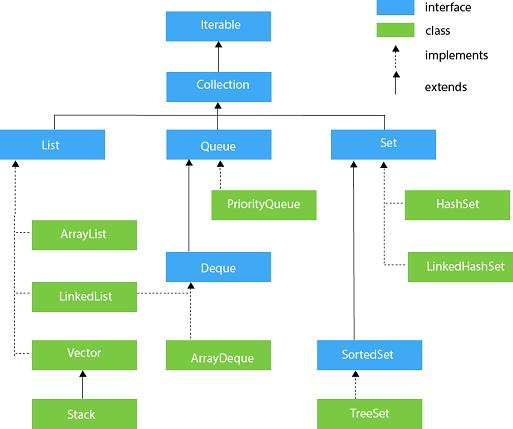
\includegraphics[width=%
0.6\textwidth]{java-collection-hierarchy}
\end{center} 

\noindent \textbf{PACCHETTI JAVA}\newline
JAVA SE $\Rightarrow$ Standard Edition \newline
JAVA EE $\Rightarrow$ Enterprise Edition \newline
JAVA ME $\Rightarrow$ Mobile Edition \newline
JAVA JDK $\Rightarrow$ linguaggio + tutte le librerie standard (java developement kit) \newline
JAVA JRE $\Rightarrow$ Solo a runtime, versione ridotta che serve solo a chi usa i programmi ma non al programmatore (java runtime enviroment) \newline
File jar  $\Rightarrow$ Archivio di tutti i pacchetti del programma \newline
JAVA JVM $\Rightarrow$ (Java virtual machine) serve per eseguire i file .jar \newline
La documentazione di java si trova on-line ed è diffusa in pacchetti che servono ad organizzare logicamente le classi, che sono organizzate in ordine alfabetico. \newline





\newpage













\newpage
\section{11-02-2019: ITERATORI E GENERICS}
\textbullet\  \textit{ITERATORE}: E' un pattern, uno stile di programmazione. Il pattern degli iteratori esiste in tutti i linguaggi ad oggetti. Con iteratore intendiamo lo scorrimento di una collezione di elementi. L'iteratore serve quindi a scorrere una collection.\newline
\textbullet\ \textit{ITERABLE}: E' una super interfaccia, e l'interfaccia \textit{COLLECTION} implementa questa super interfaccia. Iterable è super tipo di tutte le interfacce.

\noindent Se una interfaccia rappresenta una super interfaccia significa che non ha un genitore, anche se in realtà estende \textit{Object}


\noindent \textbf{MAPPA}\newline
Una mappa è una struttura dati che mappa chiavi e valori, ha quindi due parametri: il tipo della chiave e il tipo del valore. Una mappa è una \textit{collection} solo se vista come una collection di coppie. Infatti una \textit{collection} è figlia di \textit{iterable} (la posizione più alta nella gerarchia), ma una \textit{mappa} NON è figlia di \textit{iterable}
\begin{center}
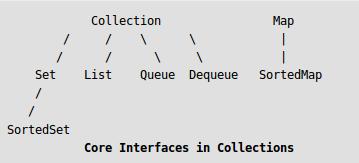
\includegraphics[width=%
0.6\textwidth]{MapInterface}
\end{center} 
Ci riferiamo ad un oggetto usando la parola \textit{sottotipo} quando esso è:\newline
\textbullet\ O una sottoclasse (extends) \newline
\textbullet\ O una sotto interfaccia (implements) \newline
Ad esempio ArrayList ha come superclasse abstract arrayList. ArrayList implementa collection. Quindi ne è sottotipo ma non sottoclasse.

\noindent \textbf{GENERICS}\newline
<? extends classe> rappresenta un tipo. \newline
<? extends E> \newline
La \textit{SUBSUMPTION} non funziona tra GENERICS. Per il parametro stesso c'è subsumption, ma non per le collection. Il tipo con il ? accetta sottotipi di parametri.\newline
\textbullet\ Il TIPO ESTERNO gode sempre della la subsumption, 
\textbullet\ Il TIPO INTERNO non gode mai della subsumption, la subsumption si può fare solo usndo i generics( quindi con <? extends E>)  \newline
[Invarianza del subtyping]: Se ciò non fosse le subsumption funzionerebbero anche nel tipo interno e questo rischierebbe la totale spaccatura \newline
Se cosi non fosse in java non verrebbero mai rispettate le regole delle classi. \newline
Java di unico ha che esiste il wildchart (?), che è un modo controllato per risolvere il problema della subsumption dei tipi interni. \newline
Prima dei generics (2003/2004) in java si programmava tutto a typecast. Per motivi di retrocompatibilità è possibile programmare in tutti e due i modi. E' comunque consigliato usare la porgrammazione con i \textit{generics}. \newline
Metodi che ritornano un booleano iniziano con sempre come se fossero domande; es: hasNext, isEmpty etc.. \newline
Un iteratore non può essere costruito con un new perchè è un'interfaccia. 
\newpage


 
\newpage
\section{15-02-2019}
\textbf{INTERFACCE}\newline
\begin{lstlisting}[basicstyle=\small,]
	public interface Iterator<T>{}
\end{lstlisting}
L'interfaccia è un contratto, nel senso che mette a disposizione una serie di metodi che ogni classe che estende quell'interfaccia deve obbligatoriamente implementare, pena un errore durante la fase di compilazione.In java quindi si può scrivere del codice ancora prima di sapere come si potrebbe implementare.

\noindent Facciamo un esempio: il "contratto" di iteratore è il seguente: \newline
\textbullet\ boolean hasNext(); \newline
\textbullet\ T next(); \newline
\textbullet\ void remove()\newline
Data una certa classe che può non essere sotto al nostro controllo non abbiamo bisogna sapere necessariamente come sono stati implementati i suoi metodi, ma ci ti basta sapere che esistono per poter dire se sia o meno un iteratore. \newline
Esempio di definizione di un metodo con iteratore come input: 
\begin{lstlisting}[basicstyle=\small,]
	public statics void scorri(Iteratore <Integer> it){
		while(it.hasnext()){
			integer n = it.next();
		}
	}
\end{lstlisting}
Esempio di utilizzo 
\begin{lstlisting}[basicstyle=\small,]
	scorri(new Iterator<>(){
		...
		...
		...
	});
\end{lstlisting}
Quest'ultima è un'espressione, o come meglio dire, un'oggetto fatto al volo. Questa sintassi è stata creata appositamente per le interfacce (dato che non si possono istanziare direttamente), senza dover andare a definire una classe con la classica implementazione dell'interfaccia. 

\noindent \textit{ANONYMOUS CLASS} meccanismo comodo per design pattern come le call-back. 

\noindent Questa implementazione garantisce che la funzione sia \textit{SOUND}, e non crasherà mai a \textit{RunTime}

\noindent \textbf{IMPLEMENTARE INTERFACCE}\newline
1) Con implements: \newline
\textbullet\ controlla i metodi che hai implementato all'interno della classe \newline
\textbullet\ assicura che siano implementati tutti 

\noindent Tipi delle interfacce \newline
Iterator $\Rightarrow$ non è un tipo \newline
Iterator<T> $\Rightarrow$ è un tipo 

\noindent \textbf{NOTAZIONE BNS} \newline
BNS è il nome della notazione e serve per poter dare delle regole grammaticali. E' una notazione che definisce la sintassi delle espressioni\newline
Iterator da solo, sintatticamente, sarebbe un tipo. Ma il compilatore verifica che non è un tipo e da errore.








\newpage 



\newpage
\section{18-02-2019: CLASSI ASTRATTE}
\textbf{CLASSE ASTRATTA} \newline
Una classe si dice astratta quando ha almeno un metodo astratto, essa serve per impedire la sua costruzione (non posso quindi istanziarla). Delle classi vengono definite astratte se anche un solo metodo è astratto. Una delle maggiori differenze tra classi astratte ed interfacce è che una classe può implementare molte interfacce ma può estendere una sola classe astratta. Una interfaccia è zucchero sintattico di una classe astratta con soli metodi astratti. Zucchero sintattico (Syntactic sugar) è un termine coniato dall'informatico inglese Peter J. Landin per definire costrutti sintattici di un linguaggio di programmazione che non hanno effetto sulla funzionalità del linguaggio, ma ne rendono più facile ("dolce") l'uso per gli esseri umani. La differenza tra classe ed interfaccia in realtà non esiste.

\noindent Un array è una struttura dati lineare, omogenea e contigua in memoria.

\noindent Per leggere una \textit{collection} si usano gli iteratori che servono per farne il get in sequenza.

\noindent \textbf{VTABLE E DIMENSIONE DI UNA CLASSE} \newline
Una virtual Table, o dispatching table, è un meccanismo utilizzato per supportare il dynamic dispatching (o anche chiamato run-time method binding).Quando una classe definisce dei metodi virtuali, il compilatore nasconde all'interno dei membri della classe una variabile che punta ad un array di puntatori a funzioni. Questi puntatori sono poi usati a runtime per invocare l'implementazione della funzione appropiata, questo perchè in compile-time non è detto che si sappia se la funzione richiamata sia quella del tipo definito o sia derivata da un'altra classe.

\begin{lstlisting}[basicstyle=\small,]
public static class Animale(){
	private int peso;
}

public static class Cane extends Animale{
	private String nome;
	public void abbaia(){};
}

public static class PastoreTedesco extends Cane{

}
\end{lstlisting}
Se costruisco un oggetto di tipo PastoreTedesco, esso sarà grande quanto un tipo int (32 bit) ed una stringa (un puntatore).
Il tutto grazie alla virtual table che tiene in memoria i puntatori dei vari campi di uno oggetto.









\newpage
\section{21-02-2019}
\par

\textit{REFLECTION} è una tecnica per conoscere i tipi e il contenuto delle classi  a runtime. \newline
Se voglio conoscere il tipo dell'enclosing class (classe che contiene) posso fare : nome.classe.this.nome \newline

\textit{BINDING} avviene anche con i tipi \newline
I parametri di una funzione sono binding nello scope della funzione.\newline
I type argument fanno binding con i type parameter, esattamente come avviene per le funzioni tra argomenti e parametri. \newline

Quando si programma con i generics si PROPAGANO. \newline

TYPE ERASURE: cancellazione dei tipi: java lo fa quando compila butta via i generics generando classi non anonime e li sostituisce con Object: il motivo è per mantenere la compatiblità con il vecchio codice che non aveva generics. Quindi i generics sono verificati dal compilatore e poi cancellati per eseguire.

















\newpage
\section{25-02-2019}
\par

Se un oggetto ha dei campi esso pesa tanto quanto la dimensione dei campi. \newline
Nei pc a 64 bit i puntatori pesano 8 byte \newline

L'ereditarietà serve anche a modificare i metodi della classe che viene ereditata. E' l'unico modo che abbiamo per modificare delle cose anche se non sappiamo cosa e chi le ha costruite. Sopratutto se non le possediamo. Un esempio è la classe ArrayList, che deve essere ereditata per implementare un motodo che ci permetta di scorrerla all'indietro. \newline


I metodi statici non si possono override perchè non sono presenti nelle virtual table (sono funzioni sciolte). \newline

Regola ereditarietà costruttore: se non definisco nessun costruttore nella sottoclasse è come se chiamassi il costruttore della superclasse SENZA parametro. 









\newpage
\section{28-02-2019: COVARIANZA e CONTROVARIANZA}
\textbf{COVARIANZA e CONTROVARIANZA DEI TIPI }\newline
Scrivendo  $C \leq A$ intendiamo che C è sottotipo di A. Definito l'operatore minore uguale passiamo alle definizioni vere e propie.

\noindent \textbf{VARIANZA} \newline
$C_{1} <\tau_{1}> \leq C_{2}<\tau_{2}> \Leftrightarrow C_{1} \leq C_{2} \bigwedge \tau_{1}\equiv \tau_{2} $
\newline
Questa regola del type system di \textit{java} ci dice che il linguaggio non è COVARIANTE, in quanto i generics non cambiano. 

\noindent \textbullet\ Esempio: ArrayList<cane> $\leq$ List<cane> (sottotipo) \newline
\textbullet\ Esempio: ArrayList<cane> $\nleq$ List<Animali> \newline
L'ultima formula non è covariante, se fosse possibile si avrebbe una doppia subsunzione sul guscio interno e sul tipo esterno \newline

\noindent \textbf{CONTROVARIANZA} \newline
Quando eredito un metodo di una classe posso sovrascriverlo usando l'overriding. Quando lo faccio un linguaggio di programmazione si dice controvariante se mi è possibile far scendere (specializzare) il tipo di ritorno, e al contempo mi è possibile far salire (rendere più generico) l'argomento di ingresso. Vediamo un esempio (\textit{NON VALIDO IN JAVA}):
\begin{lstlisting}
/* Data questa gerarchia di classi: */
  public class Cane extends Animale{
	/* nella classe Cane faccio l'override
 	 * del metodo ereditato dalla classe
 	 * Animale */  
	public Cane m(Cane c){
		return c;
	}
  }
  
 public class PastoreTedesco Extends Cane{
 	@Override
	public PastoreTedesco m(Animale c){
		return new PastoreTedesco;
	}
	/* rispetto al metodo originale
	 * il tipo di ritorno del metodo 
	 *		(PastoreTedesco) scende (sottoclassi)
 	 * il tipo del parametro di ingresso 
 	 * 		(Animale) sale (superclasse) */	
 }
\end{lstlisting}

\noindent Detto questo è bene specificare che Java supporta i solo i tipi di ritorno controvarianti, è possibile controvariare SOLO il tipo di ritorno del metodo, ed è possibile farlo solamente scendendo (sottotipo). Ed è possibile Fare questo nella fase di overriding, non in quella di overloading. In caso di overloading il tipo di ritorno deve essere lo stesso.

\noindent Il seguente è l'esempio corretto in java:
\begin{lstlisting}
public Cane m (Cane c){return c;}

@Override
public PastoreTedesco m(Cane c){return new PastoreTedesco();}
\end{lstlisting}

\noindent \textbf{SOUNDNESS IN JAVA} \newline
\textbullet\ SOUND : un programma che compila può essere eseguito senza errori \newline
\textbullet\ SOUND JAVA: un programma compila e termina, a meno di una eccezione. \newline
Un esempio di SOUND JAVA è il seguente:in java è possibile avvenga un segmentation fault non per un problema di casting, ma solamente se accediamo ad un indice di un array che non abbiamo allocato, quindi il programma termina a meno di una eccezione. Ci sono invece linguaggi dove non esistono gli array, quindi non accadrà mai segmentation fault e il codice terminerà sempre alla fine senza eccezioni, ovviamente senza fare i controlli di semantica. 

\noindent \textbf{WILDCARDS} \newline
\noindent Recentemente è stato inserito un pattern che permette anche in Java la covarianza: sono i generics con i wildcards. 
\begin{lstlisting}
Arraylist<? extends Animale> m = new List<Cane>();
\end{lstlisting}
\noindent Da questo si capisce che la covarianza può essere usata, ma solamente se esplicitata con il wildcard. \newline
Sono molto usati perchè i wildcard non sono tipi del primo ordine, infatti il \textit{tipo} "? extends classe" non esiste!!!Non posso definire una variabile come segue: 
\begin{lstlisting}
? extends Animale m = new Cane();
/* questa sintassi si può usare solo come type argument */
\end{lstlisting}
Significato: permettono la covarianza, sono tipi temporanei che non possono essere scritti nel codice, però possono essere subsunti con il get(). \newline
Un altro DESIGN PATTERN: callback

















\newpage
\section{4-03-2019: CLASSI ANONIME, LAMBDA E FUNZIONI ORDINE SUPERIORE}
\textbf{DESIGN PATTERN} \newline
\textbullet\ Iteratore \newline
\textbullet\ Compact o Callback o Unary function 

\noindent \textbf{CLASSI ANONIME} \newline
Le classi \textit{lambda} servono per fare funzioni al "volo",senza quindi avere il bisogno di implementare delle interfacce in classi separate. Vediamone un esempio:

\begin{lstlisting}[basicstyle=\small,]
interface HelloWorld {
	public void greet();
    public void greetSomeone(String someone);
}

public static void main (String args[]) {
    HelloWorld frenchGreeting = new HelloWorld() {
        String name = "tout le monde";
        public void greet() {
            greetSomeone("tout le monde");
        }
        public void greetSomeone(String someone) {
            name = someone;
            System.out.println("Salut " + name);
        }
    };
}

\end{lstlisting}

\noindent \textbf{LAMBDA ASTRAZIONI} \newline
Le espressioni \textit{lambda} servono per fare funzioni al "volo",senza quindi avere il bisogno di implementare delle interfacce in classi separate, classi anonime e classi innestate. Si ricorda che le espressioni lambda possono essere usate solo per implementare interfacce funzionali (cioè interfacce che possiedono un solo metodo astratto). Vediamone un esempio:

\begin{lstlisting}[basicstyle=\small,]
interface MyString {
	String myStringFunction(String str);
}

public static void main (String args[]) {
	MyString reverseStr = (str) -> {
		String result = "";		
		return result;
	};
	reverseStr.myStringFunction("temp");
}
\end{lstlisting}

\noindent \textbf{FUNZIONI DI ORDINE SUPERIORE} \newline
Sono delle funzioni che prendono delle funzioni come parametri di ingresso 
\begin{lstlisting}[basicstyle=\small,]
/* questa interfaccia è equivalente all'interfaccia java.util.Functional
 * essa infatti espone una serie di funzioni, senza implementazione, tra 
 * cui anche le call-back */
public interface Func<A, B>{
	B execute(A a); 
	
	/* questa è l'unica funzione esposta dall'interfaccia
	 * un altro nome ragionevole per il metodo execute() è apply() 
	 * oppure call() il nome deve ricordare il fatto di richiamare 
	 * la funzione  */
}

/* questa funzione va ad utilizzare la funzione Func definita sopra */
public static <A,B> List<B> map(List<A> I, Func<A,B> f){
	List<B> r = new ArrayList<>();
	for(A x: l)
		r.add(f.execute(x));
	return r;

}
\end{lstlisting}
A e B sono \textit{generics} locali al metodo(e solo al metodo) \newline
I generics sulle classi servono per parametrizzare, non per fare polimorfismo \newline
\begin{lstlisting}[basicstyle=\small,]
public static <A,B> List<B> map(List<A> I, Func<A,B> f){
/* dove in "public static <A,B>" dichiaro i parametri che useremo
 * mentre in "List<a> .. Func <A,B>" "uso" i parametri */
\end{lstlisting}

\noindent Funzione FILTER: 
\begin{lstlisting}[basicstyle=\small,]
/* questa funzione è simile alla funzione Func definita sopra
 * solo che rende più chiaro il suo scopo: filtrare degli elementi
 * da aggiungere in una lista */
public static <A> List<A> Filter (List<A> l, Func<A,Boolean> p){
	List<A> r = new ArrayList<>();
	for(A x : l)
		if(p.execute(x))
			r.add(x);
	return r;
}
\end{lstlisting}

\noindent La seguente \textit{Filter2} NON funziona perché usa la \textit{remove()} delle Collection, ma non è possibile rimuove un elemento in fase di scorrimento (è scritto nella documentazione)

\begin{lstlisting}[basicstyle=\small,]
public static <A> void Filter2 (List<A>, Func<A, Boolean> p){
	for(A a: l)   /* il for each in Java essere zucchero sintattico */
		if(p.execute(a))
			l.remove(a);

}
\end{lstlisting}
Se non posso rimuovere come ho fatto sopra un elemento posso invece chiedere all'iteratore di rimuovere l'elemento stesso, esso rimuoverà quello a cui stiamo puntando. Quindi invece di usare un ciclo for come sopra, uso l'iteratore per scorrere la lista usando in metodo \textit{hasNext}.

\begin{lstlisting}[basicstyle=\small,]
/* questo funziona perchè chiama la remove() dell'iteratore
 * mentre prima chiamavo il remove della lista */
public static <A> void Filter2 (List<A>l, Func<A, Boolean> p){
	Iterator<A> it = l.iterator();
	while(it.hasNext()){
		A a = it.next();
		if(!(p.execute(a)))
			it.remove();
	}
}

/* volendo posso usare le funzionalita delle nuove API FUNZIONALI
 * l.removeIf(a -> !p.execute(a)); */
\end{lstlisting}

\noindent Posso usare Function<A,B> di java come funziona Func? \newline
Esempio di chiamata:

\begin{lstlisting}[basicstyle=\small,]
public static void main(String argv[]){
	List<String> strings = new ArrayList<>();
	string.add("ciao");
	string.add("pippo");
	string.add("unive");
	/* voglio calcolare la lunghezza della mia lista */
	List<Integer> r = map(strings, new Func<String, Integers>{ 
	
		/* "String" è la lista, "Integers" è la funzione
         * In realtà devo passare un oggetto di tipo Func<>
         * alla funzione map, perciò passo una classe anonima,
         * all'interno della quale trovo solo un metodo
         * (che ha la stessa firma del metodo dell'interfaccia Func)*/
         
		@Override 
		public Integer execute(String a){
			return a.length();
		}	
	});
}
\end{lstlisting}


\noindent La seguente funzione data una lista di interi scarta gli elementi minori di zero: questo è il modo per non usare un for con un ciclo if innestato.

\begin{lstlisting}[basicstyle=\small,]
public static void main__filter(){
	 List<Integer> interi  = new ArrayList<>();
	 interi.add(89);
	 interi.add(34);
	 interi.add(-16);
	 interi.add(560);
	 interi.add(-1);
	 interi.add(46);
	 /* filter prende una lista e un predicato e produce una lista in uscita */
	 List<Integer> l = Filter(ints, new Func<Integer, Boolean>(){
	 	@Override
	 	public Boolean execute (Integer a){
	 		return a>=0;
	 	}
	 });
}
\end{lstlisting}

\noindent Oppure 

\begin{lstlisting}[basicstyle=\small,]
	Filter2 (interi , new Func<Integer, Boolean>(){
		@Override
		public Boolean execute (Integer a)
			return a>=0;
	})
\end{lstlisting}

\noindent \textbf{GENERICS LOCALI (Polimorfismo parametrico di primo ordine)} 

\begin{lstlisting}[basicstyle=\small,]
    public static Object ident__ugly(Object o) {
        return o;
    }   
    /* con un metodo di subtyping che è POLIMORFISMO VERTICALE, 
     * questa funzione NON è SOUND perché sono costretto a 
     * fare un CAST di ciò ciò che ricevo */

    public static <X> X ident(X x) {
        return x;
    }   
    /* con i generics, che è POLIMORFISMO PARAMETRICO, non
     * devo più fare nessun cast. Sono sicuro del tipo di
     * ritorno */
\end{lstlisting}

\begin{lstlisting}[basicstyle=\small,]
	public static void main__ident	(){
		Cane fido = new Cane();
		Cane c = (Cane) ident__ugly(fido); /* ritorna un cane 
											* facendo un cast */
		Cane c2 = ident(fido);  /* ritorna un cane senza dover 
								 * fare un fast */ 
		Gatto g = ident(new Gatto());
	}
\end{lstlisting}
























\newpage
\section{7-03-2019}
I tre tipi possibili di wildcards sono: \newline
\textbullet\ <?> top type \newline
\textbullet\ <? extends nametype> \newline
\textbullet\ <? super nametype > \newline



\begin{lstlisting}[basicstyle=\small,]

List<?> l1 = new ArrayList<Cane>();
\\ ? -> Da solo significa che indica un tipo che gerarchicamente
\\ e piu in alto di Object, viene detto top type

l1.get(int index) \\ritorna un capture of ? , qualcosa che sia figlio del top type 

\end{lstlisting}

\noindent Il tipo ? non può essere usato come tipo per una variabile, ? x non si può fare, però posso fare
Object x = l1.get(..) \newline
Mentre ? extends Animale -> qualsiasi cosa che sia figlio di animale \newline
l2.get(0) -> ritorna un capture of ? extends Animale -> qualsiasi cosa figlia di animale (posso però fare Binding di qualcosa che sia al massimo Animale) \newline

\begin{lstlisting}[basicstyle=\small,]

	List<Animale> t3 = new ArrayList<Gatto>();
	// essere errato, si puo subscrivere solamente il guscio esterno, la versione corretta essere fatta con il 
	// wildcard
	
	List<? extends Animale> t3 = new ArrayList<Gatto>();

\end{lstlisting}

\noindent Posso subsumero solo il tipo esterno, se voglio subsumere anche il tipo interno devo usare le wildcards. \newline

\noindent Il caso simmetrico è il seguente: \newline
? super Animale -> qualcosa che sia più su di Animale (più generale) \newline
In questo caso posso passare animale a tutto quello che sta sopra
l2.add(new Animale) -> ?? non compila perchè... \newline





\noindent Riprenderemo la map vista l'altra volta. Ad esempio, per trasformare animali in piante: 

\begin{lstlisting}[basicstyle=\small,]

public static class Vegetale{}

public static void main_map(){
	List<cani> l1 = new ArrayList<>();
	List<Vegetali> l2 = map(l1, new func<Animale, Vegetale>(){
		@Override
		public Vegetale execute(Animale a){
			return null;
		}
	
	});
}

\end{lstlisting}

\noindent Questo non compila in quanto i generics non sono soggetti alla subsumption. \newline
Per farlo compilare modifichiamo la funzione map: 

\begin{lstlisting}[basicstyle=\small,]

public static  <x, y> List<x> map(List<x>, Func(? super <x, y> f)){
...

}

\end{lstlisting}

\begin{lstlisting}[basicstyle=\small,]

    public static <X, Y> List<Y> map(List<X> l, Func<? super X, ? extends Y> f) {
        List<Y> r = new ArrayList<>();
        for (X x : l) {
            r.add(f.execute(x));
        }
        return r;
    }
    
\end{lstlisting}

Questa è la versione più generale possibile. \newline


\noindent \textbf{NESTED CLASS}\newline
La Nested Class (o Inner Class) è totalmente senza relazione rispetto alla enclosed class (outer class).\newline
Nel caso precedente main{\_}functional è la enclosed class, in quanto sto lavorando su quella. \newline
Le nested class vedono i campi della enclosing class, ma se sono statiche non vedono i campi. 


Normalmente le nested class vedono il "this" della classe che le contiene (outer class), se pero sono statiche non vede il this.






\noindent \textbf{OVERLOADING} \newline
Permette di definire metodi con stesso nome ma firma diversa. 



\begin{lstlisting}[basicstyle=\small,]


public static class c{
	public int m(){
		return 1;
	}
	public int m(int x){
		return x+1;
	}
	public int m(float x){
		return (int)(x-1.0f);
	}
	public int m(int x, int y){
		return x+y;
	}		
}

\end{lstlisting}

\noindent L'overloading non è permesso cambiando il tipo di ritorno e lasciando il resto inalterato. Devono essere diversi i parametri! \newline
-ordine \newline
-tipi \newline
-numeri \newline

\noindent L'overloading è del tutto gestito dal compilatore.

\begin{lstlisting}[basicstyle=\small,]


public Number m(Number x){
	return x;
}

\end{lstlisting}

























\end{document}